\documentclass[tikz]{standalone}

\usetikzlibrary{matrix, positioning, automata, arrows}

\begin{document}

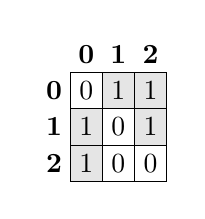
\begin{tikzpicture}[
    2d-arr/.style={matrix of nodes, row sep=-\pgflinewidth, column sep=-2*\pgflinewidth, nodes={draw}},
    row 1/.style={nodes={draw=none}},
    column 1/.style={nodes={draw=none}}
  ]

  \matrix (K) [2d-arr, nodes={draw}] {
      & \textbf 0 & \textbf 1 & \textbf 2 \\
    \textbf 0 & 0 & |[ fill=gray!20]| 1 & |[ fill=gray!20]| 1  \\
    \textbf 1 & |[ fill=gray!20]| 1 & 0 & |[ fill=gray!20]| 1 \\
    \textbf 2 & |[ fill=gray!20]| 1 & 0 & 0 \\
  };

\end{tikzpicture}

\end{document}